\documentclass[12pt,a4paper]{article}
\usepackage[utf8]{inputenc}
\usepackage[german]{babel}
\usepackage[T1]{fontenc}
\usepackage{amsmath}
\usepackage{amsfonts}
\usepackage{amssymb}
\usepackage{graphicx}
\usepackage{siunitx}
\usepackage{float}
\usepackage[left=2cm,right=2cm,top=2cm,bottom=2cm]{geometry}
\usepackage{hyperref}
\author{Gerald}


\begin{document}
\sisetup{separate-uncertainty = true}
	\setlength{\parindent}{0pt} 
	\begin{center}
		{\LARGE Versuchsprotokoll}\\
		\begin{large}
			zum Fortgeschrittenenpraktikum im Bachelorstudiengang Physik\\[0.4cm]
			an der RWTH Aachen\\
			II. Physikalisches Institut A\\[5.5cm]
			\Large\textbf{\textsl{Röntgenspektroskopie (T06)}}\\[5.5cm]
			\normalsize\textit{vorgelegt\\von}\\[0.4cm]
			\large{Moritz Berger (355244)\\Gerald Kolter (355005)}\\\textbf{Gruppe 30}\\[2cm]
			\large \textbf{Wintersemester 2017/18}
		\end{large}
	\end{center}
	\newpage
	
	\tableofcontents
	\newpage
	
\section{Hintergund}
Wenn man Materialien mit hochenergetischen Teilchen bestrahlt, so wechelwirken diese folgendermaßen mit den darin enthaltenden Atomen\footnote{Quelle:}:
\begin{enumerate}
\item Bei der Bewegung durch das Material werden die Teilchen abgebremst. Die dabei freiwerdende Energie äußert sich als ein kontinuirliches elektromagnetisches Spektrum, das Bremsstrahlung genannt wird. Die Intensität dieser Strahlung nimmt mit der Masse der abgebremsten Teilchen ab.
\item Die Teilchen geben ihre Energie an ein Elekron im Atom ab, was infolgedessen ionisiert wird. Dadruch wird eine Elektronposition frei und ein höherenergetisches Elektron im Atom kann auf diese Position fallen, wobei ein Röntgenquant abgestrahlt wird. Diesem Übergang kann eine diskrete Energie zugeordent werden. In der Realität äußert er sich wegen Energieunsicherheiten als Gau
\end{enumerate}
Der zweite Effekt hängt direkt von dem Atomaufbau ab, wodurch sich das dadurch ausgestrahlte Spektrum je nach Element unterscheidet. Dadurch kann man die Zusammensetzung eines Materials untersuchen, was in diesem Versuch ausgenutzt wird.
In diesem Versuch wird sowohl ein $\alpha$-Strahler, als auch eine Röntgenquelle als Quelle der hochenergetischen Teilchen benutzt.\\
Ziel ist es, beide Aufbauten mithilfe von mehreren Proben bekannter Zusammensetzung zu kalibrieren, um dann eine Reihe von unbekannten Proben mithilfe ihrer Röntgenpeaks zu untersuchen.
\section{Aufbau}
\subsection{$\alpha$-Quelle}
Der erste Aufbau besteht einem X-123 Spektrometer, welches aus einem Halbleiterdetekor der Kennung XR100CR und einem digitalen Pulsprozessor DP5 besteht, der die vom Detektor regristrierten Signale verstärkt und digitalisiert. Der Detektor kann maximal Energien von c.a \SI{60}{keV} aufnehmen, da Teilchen mit größerer Energie den Detektor durchfliegen.\\
Diese Signale werden an einen PC weitergeleitet, wo sie mit dem Programm und der Software ADMCA\footnote{\url{http://amptek.com/products/dpp-mca-display-acquisition-software/}} mithilfe eines Multi-Channel-Analyzers (MCA) nach ihrer Energie auf 496 Kanäle aufgeteilt werden.\\
Zur Kalibration dieser Channels gegen die Energie wird eine variable Röntgenstrahlquelle der Kennung 0317LA benutzt, welche aus einer $^{241}AM$-Quelle besteht, die $\alpha$-Strahlung auf ein durch eine Drehscheibe variables Target strahlt. Diese Quelle wird direkt vor den Detektor gestellt.\\
Zur Aufnahme von unbekannten Proben wird eine $^{241}AM$-Quelle der Kennummer Z3715 benutzt, welche in eine Bleibefestigung eingelassen wird.
\subsection{Röntgenquelle}
Bei den Messungen mit der Röntgenquelle wird ein X-123 Spektrometer der gleichen Bauart wie oben beschrieben verwendet. Die Röntgenquelle hat die Kennnummer BJ8288.
\section{Durchführung}
\subsection{$\alpha$-Quelle}
Als erstes muss über eine Kalibration den Channels eine Energie zugeordent werden.\\
Die dafür benutzte variable Röntgenstrahlquelle besitzt 6 Targets aus verschiedenen Materialien: Cu, Rb, Mo, Ag, Ba und Tb.\\
Bevor die Messungen gestartet werden können, muss an dem benutzten Programm der richtige Messbereich eingestellt werden. Dies geschieht an dem Tb Spektrum, da diese Probe Röntgenstrahlung mit der größten Energie aussendet, welche außerdem knapp unterhalb der maximal messbaren Energie liegt.\\
Dazu wird in den Programmeinstellungen der Verstärkungsfaktor so eingestellt, dass die Linie mit der größten Energie möglichst weit rechts im sichtbaren Spektrum liegt.\\
Außerdem kann über den Reiter shaping eine Pile-up Rejection(PUR) und eine Rise Time Discrimination(RTD) zugeschaltet werden. Bei einer Schnellauswertung haben diese Einstellungen aber keinen nennenswerten Unterschied gemacht, weswegen sie für die Messungen deaktiviert wurden.\\
Alle Einstellung sind in Tabelle \ref{tab:alpha_Einstellungen} aufgelistet.\\
\\
Nun wird für jede der sechs Proben über \SI{15}{min} das Spektrum aufgenommen.\\
Danach werden für eine Edelstahlplatte und mehrere Münzen ebenfalls über \SI{15}{min} die Spektren aufgenommen.
\begin{table}
\centering
\begin{tabular}{|c|c|}
\hline 
Einstellung & Wert \\ 
\hline 
Gain(coarse) & 2.1x \\ 
\hline 
Gain(fine) & 0.95 \\ 
\hline 
RTD & aus \\ 
\hline 
PUR & aus \\ 
\hline 
Messzeit & 15 min \\ 
\hline 
\end{tabular} 
\caption{Einstellungen für die Messungen mit der $\alpha$-Quelle.}
\label{tab:alpha_Einstellungen}
\end{table}
\subsection{Röntgenquelle}
\begin{table}
\centering
\begin{tabular}{|c|c|}
\hline 
Einstellung & Wert \\ 
\hline 
Hochspannung & \SI{50}{kV} \\ 
\hline 
Strom & \SI{70}{\mu A} \\ 
\hline 
Gain & 23.8 \\ 
\hline 
PUR & aus \\ 
\hline 
Messzeit & \SI{5}{min} \\ 
\hline 
\end{tabular} 
\caption{Einstellungen für die Messungen mit der Röntgenquelle.}
\label{tab:röntgen_Einstellungen}
\end{table}

Die unverändert übernommenen Einstellungen sind in Tabelle \ref{tab:röntgen_Einstellungen} aufgelistet. \\
Auch hier muss zunächst eine Kalibration der Channels gegen die Energie durchgeführt werden. Dazu werden I, Cu, Ag und der bereits mit der $\alpha$-Quelle untersuchte Stainless Steel verwendet. \\
Anschließend werden folgende Messreihen aufgenommen:
\begin{enumerate}
\item Sechs verschiedene unbekannte Proben: Ein Computerchip, ein Magnet, ein Block Blei, eine jugoslawische 2-Dinar-Münze, eine 10-Pfennig-Münze und eine 10-Rubel-Münze
\item Mit dem Stainless Steel wurde eine Messreihe mit variierter Spannung an der Röntgenröhre aufgenommen. Die eingestellten Spannung sind: \SI{20}{kV}, \SI{35}{kV} und \SI{50}{kV}
\item Mit dem Blei Block wurde eine Messung mit und eine ohne eingeschalteter PUR aufgenommen  
\end{enumerate}

\section{Ergebnisse $\alpha$-Quelle}
\subsection{Kalibration}

\begin{figure}
\centering
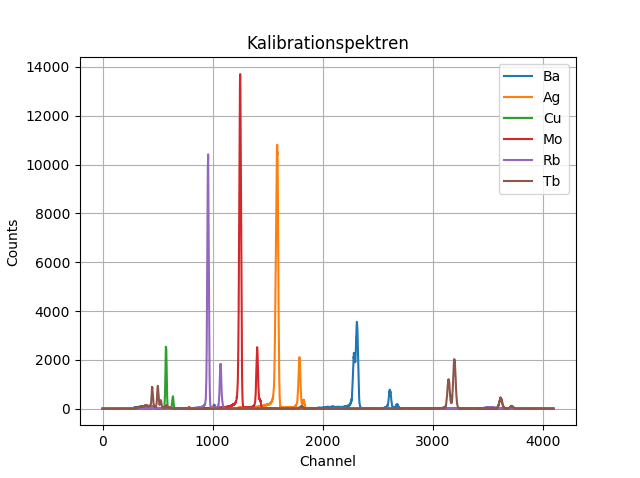
\includegraphics[scale=0.9]{Bilder/alpha/kal_alles.png}
\caption{Alle für dei Kalibration aufgenommenen Spektren.}
\label{fig:kal_alles}
\end{figure}

Die Spektren der sechs Proben sind in Abbildung \ref{fig:kal_alles} gezeigt.\\
Da das Rauschen in den Daten nicht sehr groß ist wird auf einen Frequenzcutoff verzichtet.\\
Für alle Spektren ist der $K_{\alpha}$ und der $K_{\beta}$ Peak zu sehen.
Nun wird an diese Peaks ein Gaussfit angepasst. Dies ist in Abbildung \ref{fig:kal_fits} beispielhaft gezeigt. Die restlichen Anpassungen befinden sich im Anhang.\\
Bei Peaks mit höheren Energien wird die Feinstrukturaufspaltung immer sichtbarer, bis man die Linien eindeutig trennen kann, wie in Abbildung \ref{fig:kal_fein} anhand des Barium $K_{\alpha}$-Peaks zu sehen. Da sich die beiden Linien aber immernoch überlagern, ist die sichtbare Position der Peaks leicht versetzt. Um die wahre Position bestimmen zu können, wird eine doppelte Gaußfunktion angefittet, die die Positionen beider Peaks bestimmt.\\
Die Feinstruktur tritt natürlich auch bei den niedrigenergetischen Peaks auf. Hier äußert sie sich dadurch, dass der Peak nicht exakt gaussförmig ist,sondern eine unterschiedliche Flankensteigung auf beiden Seiten hat. Dadurch verschiebt sich die Position leicht, wenn man den Anpassungsbereich vergrößert.\\
Um den Fehler auf die Position besser abschätzen zu können, wird deswegen einmal ein kleiner und einmal ein großer Bereich an die Peaks angepasst. Der Unterschied in der Peakposition wird als Fehler angenommen, solange dieser größer als der Fitfehler ist.\\
Als Peakposition wird immer die mit dem kleineren Fehler genommen, da dise den jeweiligen Peak genauer beschreibt.\\
\\
An den so bestimmten Peaks wird nun eine Energiekalibration durchgeführt. Dazu wird den Peaks eine Energie zugeordnet, die den Literaturwerten entnommen wurde, welche in Tabelle \ref{tab:alpha_lit} aufgelistet sind. Falls in einem Peak mehrere Literaturwerte liegen, so wird der Wert genommen, dessen Peak die höhere Intensität hat. Dies ist immer $K_{\alpha_1}$ und $K_{\beta_{1}}$.\\
Nun wird eine lineare Regression durchgeführt, die den Channels eine Energie zuweist. Dies ist in Abbildung \ref{fig:kal_linreg} zu sehen. Daraus ergibt sich eine Kalibrationsgrade von
\begin{equation}
E = (0.013904\pm0.000004)\cdot CH + (0.060\pm0.010)
\end{equation}
wobei die Energie in keV angegeben wird.

\begin{table}
\centering
\begin{tabular}{|c|c|c|c|c|}
\hline 
Probe & $K_{\alpha_1}$ & $K_{\alpha_2}$ & $K_{\beta_2}$ & $K_{\beta_{1/3}}$ \\ 
\hline 
Cu & $576.8\pm0.2$ & - & -& $638.5\pm0.6$\\ 
\hline 
Rb & $958.1\pm0.1$ & - & -& $1071.5\pm0.4$\\ 
\hline 
Mo & $1249.8\pm1.5$ & - & $1430.0\pm0.9$ & $1404.1\pm0.4$ \\ 
\hline 
Ag & $1588.7\pm1.0$ & - & $1825.1\pm0.2$ & $1787.5\pm0.3$ \\ 
\hline 
Ba & $2310.1\pm0.8$ & $2282.8\pm0.9$ & $2674.6\pm0.2$ & $2609.4\pm0.3$ \\ 
\hline 
Tb & $3195.4\pm0.2$ & $3152.7\pm0.1$ & $3715.4\pm0.4$ & $3616.1\pm0.4$ \\ 
\hline 
\end{tabular} 
\caption{Peakpositionen in den Channels der abgelesenen Peaks. Falls keine Feinstrukturaufspaltung ermittelt werden konnte, wurd angenommen, dass der Peak immer der mit der größeren Intensität ist.}
\label{tab:alpha_kal}
\end{table}

\begin{table}
\centering
\begin{tabular}{|c|c|c|c|c|c|}
\hline 
Probe & $K_{\alpha_1}$ & $K_{\alpha_2}$ & $K_{\beta_2}$ & $K_{\beta_{1}}$ & ($K_{\beta_{3}}$) \\ 
\hline 
Cu & 8,047.8 & 8,027.8 & - & 8,905.3 & 8,905.3\\ 
\hline 
Rb & 13,395.3 & 13,335.8  & 15,185 & 14,961.3 & 14,951.7\\ 
\hline 
Mo & 17,479.3 & 17,374.3 & 19,965.2  & 19,608.3 & 19,590.3\\ 
\hline 
Ag & 22,162.9 & 21,990.3 & 25,456.4 & 24,942.4 & 24,911.5\\ 
\hline 
Ba & 32,193.6 & 31,817.1 & 37,257 & 36,378.2 & 36,304.0\\ 
\hline 
Tb & 44,481.6 & 43,744.1 & 51,698 & 50,382 & 50,229\\ 
\hline 
\end{tabular} 
\caption[test]{Literaturwerte\footnotemark für die Peakpositionen. Alle Angaben sind in eV, wobei nach der 1000eV stelle ein Komma steht.}
\label{tab:alpha_lit}
\end{table}
\footnotetext{Quelle: \url{http://xdb.lbl.gov/Section1/Table_1-3.pdf}}

\begin{figure}
\centering
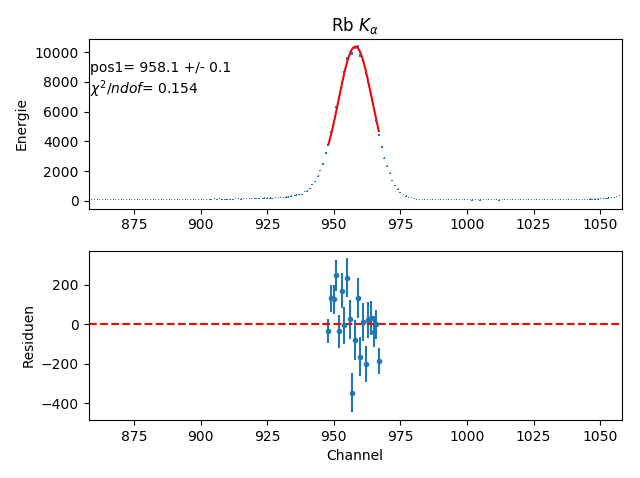
\includegraphics[scale=0.8]{Bilder/alpha/rb_alpha_1.png}
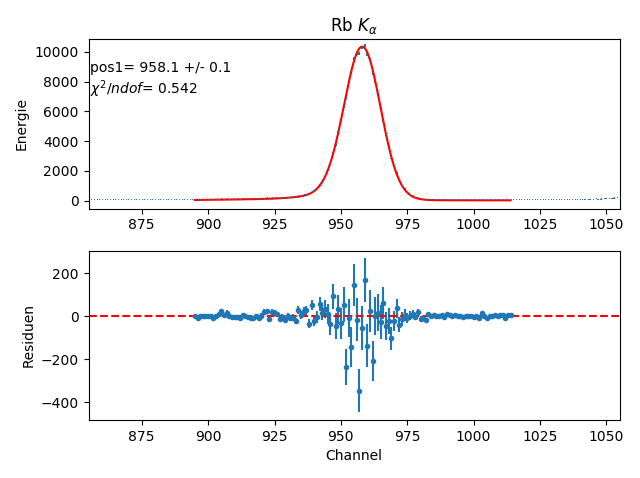
\includegraphics[scale=0.8]{Bilder/alpha/rb_alpha_2.png}
\caption{Beispiel für den Gaußfit anhand des $K_{\alpha}$ Peaks von Rubidium. In diesem Peak liegen $K_{\alpha_1}$ und $K_{\alpha_1}$ sehr eng nebeneinander, weswegen der Peak gaussförmig ist und sich die Position bei Vergrößerung kaum verändert}
\label{fig:kal_fits}
\end{figure}

\begin{figure}
\centering
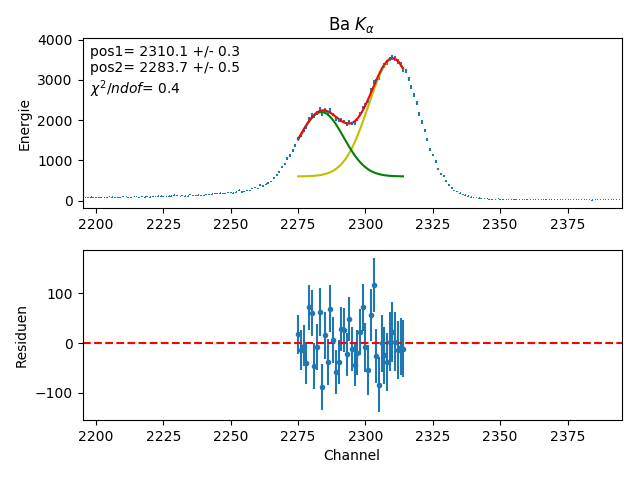
\includegraphics[scale=0.8]{Bilder/alpha/ba_alpha_1.png}
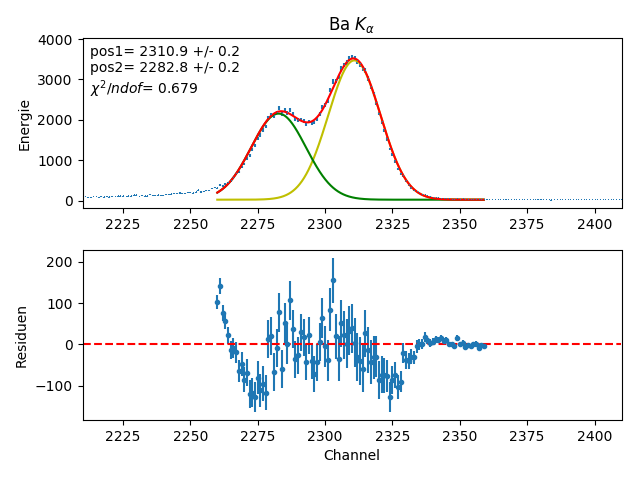
\includegraphics[scale=0.8]{Bilder/alpha/ba_alpha_2.png}
\caption{Doppelter Gaussfit (in rot) an sich überlappende Peaks. Bei der Änderung des Fitbereiches ändert sich auch die Positionder Peaks. Es sind außerdem die beiden einzelnen Peaks eingezeichnet (gelb und grün).}
\label{fig:kal_fein}
\end{figure}

\begin{figure}
\centering
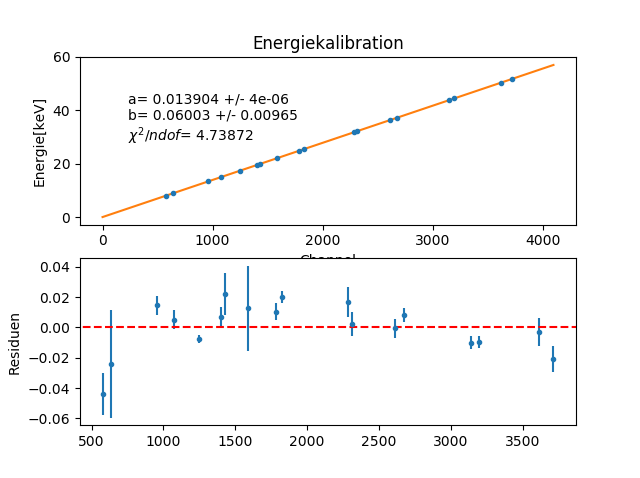
\includegraphics[scale=0.8]{Bilder/alpha/kal.png}
\caption{Lineare Regression an den Channelpositionen und der zugewiesenen Energie. Der jeweilige Fehler der Datenpunkte ist der Maximalfehler aus Fit und Fitvariation.}
\label{fig:kal_linreg}
\end{figure}

\subsection{Auswertung unbekannter Proben}
\subsection{Energieauflösung}

\begin{table}
\centering
\begin{tabular}{|c|c|}
\hline 
Peakenergie [\si{keV}] & Full Width Half Maximum [\si{keV}] \\ 
\hline
8.078 $\pm$ 0.010 & 0.243 $\pm$ 0.023 \\ 
\hline
8.929 $\pm$ 0.010 & 0.262 $\pm$ 0.023 \\ 
\hline
13.356 $\pm$ 0.010 & 0.320 $\pm$ 0.023 \\ 
\hline
14.956 $\pm$ 0.010 & 0.372 $\pm$ 0.023 \\
\hline
17.395 $\pm$ 0.010 & 0.382 $\pm$ 0.023 \\ 
\hline
19.583 $\pm$ 0.010 & 0.327 $\pm$ 0.023 \\ 
\hline
19.943 $\pm$ 0.010 & 0.319 $\pm$ 0.023 \\ 
\hline
22.041 $\pm$ 0.010 & 0.453 $\pm$ 0.023 \\ 
\hline
24.914 $\pm$ 0.010 & 0.363 $\pm$ 0.023 \\
\hline
25.436 $\pm$ 0.010 & 0.343 $\pm$ 0.023 \\
\hline
31.799 $\pm$ 0.010 & 0.393 $\pm$ 0.023 \\ 
\hline 
32.191 $\pm$ 0.010 & 0.378 $\pm$ 0.023 \\ 
\hline
36.341 $\pm$ 0.010 & 0.456 $\pm$ 0.023 \\ 
\hline
37.249 $\pm$ 0.010 & 0.448 $\pm$ 0.023 \\  
\hline
43.754 $\pm$ 0.010 & 0.442 $\pm$ 0.023 \\ 
\hline
44.489 $\pm$ 0.010 & 0.430 $\pm$ 0.023 \\ 
\hline
50.333 $\pm$ 0.010 & 0.543 $\pm$ 0.023 \\ 
\hline
51.718 $\pm$ 0.010 & 0.520 $\pm$ 0.023 \\ 
\hline
\end{tabular} 
\caption{Peakenergie und zugehörige Full Width Half Maxima.}
\label{tab:alpha_energieaufloesung}
\end{table}

Zur Bestimmung der Energieauflösung werden die Peaks verwendet, die auch zur Kalibration verwendet werden. Dabei werden die Gaußanpassungen an die Peaks nach der Umrechnung der Kanäle auf Energie. Das Full Width Half Maximum (FWHM) bestimmt sich aus dem Breitenparameter aus der Gaußanpassung $\Delta$ gemäß:
\begin{equation*}
\textrm{FWHM} = 2 \cdot \sqrt{2 \cdot \ln(2)} \cdot \Delta
\end{equation*}
Entsprechend berechnet sich der Fehler über:
\begin{equation*}
\sigma _\textrm{FWHM} = 2 \cdot \sqrt{2 \cdot \ln(2)} \cdot \sigma _\Delta
\end{equation*}
Die Fehler auf die Breitenparameter und die Peakpositionen kommen aus der Anpassung. \\
Wegen des erwarteten Zusammenhangs $\Delta E \propto \sqrt{E}$ wird die Energieauflösung $\Delta E$ gegen die Wurzel der Energie aufgetragen. Der Fehler bestimmt sich zu:
\begin{equation*}
\sigma _{\sqrt{E}} = \dfrac{\sigma _E}{2 \cdot \sqrt{E}}
\end{equation*}
Tabelle \ref{tab:alpha_energieaufloesung} zeigt die dadurch entstehenden Datenpunkte. An diese Punkte kann nun zur Überprüfung des Zusammenhang eine Transformation und dann eine lineare Regression durchgeführt werden. Diese ist in Abbildung \ref{fig:alpha_energieaufloesung} gezeigt. Das $\chi ^2$/ndof von 2.98 deutet auf eine verhältnismäßig gute Anpassung, sodass der Zusammenhang $\Delta E \propto \sqrt{E}$ als bestätigt betrachtet werden kann.

\begin{figure}
\centering
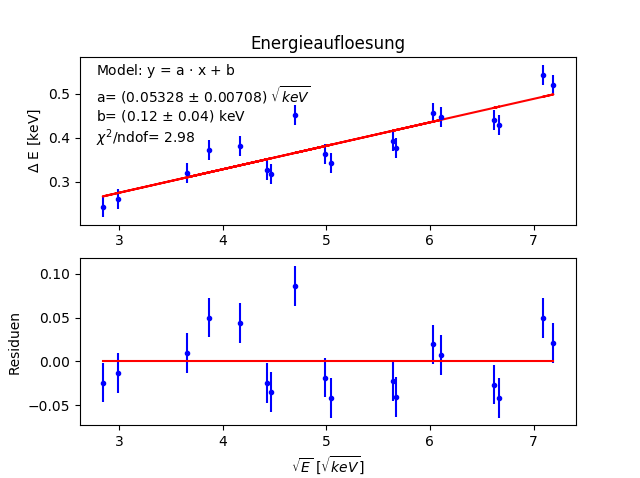
\includegraphics[scale=0.8]{Bilder/Energieaufloesung/alpha_gesamt.png}
\caption{Lineare Regression an die Full Width Half Maxima und die Energien der Peaks.}
\label{fig:alpha_energieaufloesung}
\end{figure}

\section{Ergebnisse Röntgenquelle}
\subsection{Kalibration}
\begin{figure}
\centering
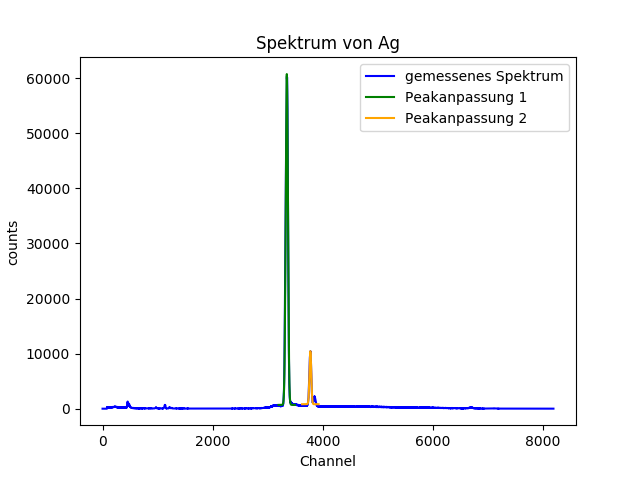
\includegraphics[scale=0.8]{Bilder/roentgen/Kalibration/Ag_gesamt.png}
\caption{Gemessenes Spektrum mit der Silberprobe.}
\label{fig:röntgen_AgSpektrum}
\end{figure}

\begin{table}
\centering
\begin{tabular}{|c|c|c|}
\hline 
Probe & Peak 1 & Peak 2 \\ 
\hline 
Ag & $3347.5\pm0.7$ & $3774.9\pm0.3$ \\ 
\hline 
Cu & $1219.6\pm0.1$ & $1349.6\pm0.7$ \\ 
\hline 
I & $4328.6\pm1.6$ & $4884.5\pm0.2$ \\ 
\hline 
Stainless Steel & $2643.0\pm0.4$ & $2969.6\pm0.9$ \\ 
\hline 
\end{tabular} 
\caption{Peakpositionen in den Channels der abgelesenen Peaks. Falls keine Feinstrukturaufspaltung ermittelt werden konnte, wurde angenommen, dass der Peak immer der mit der größeren Intensität ist.}
\label{tab:röntgen_kal}
\end{table}

Abbildung \ref{fig:röntgen_AgSpektrum} zeigt beispielhaft das gemessene Spektrum der Silberprobe. \\
Da das Rauschen in den Daten sehr gering ist, wurde auf einen Tiefpassfilter verzichtet. \\
Zur Bestimmung der Peakpositionen werden Gaußfunktionen an die Peaks gefittet. Für den Fehler auf die Position werden diese Fits mit zwei unterschiedlichen Fitbereichen durchgeführt. Die Position ist dann der Mittelwert und der Fehler die Differenz der beiden Ergebnisse. Tabelle \ref{tab:röntgen_kal} zeigt die bestimmten Peakpositionen. Beim Stainless Steel wurden nur Peaks betrachtet, die mit der $\alpha$-Quelle eindeutig bestimmt werden konnten.

\begin{table}
\centering
\begin{tabular}{|c|c|c|c|c|c|}
\hline 
Probe & $K_{\alpha_1}$ & $K_{\alpha_2}$ & $K_{\beta_2}$ & $K_{\beta_{1}}$ & ($K_{\beta_{3}}$) \\ 
\hline 
Ag & 22,162.9 & 21,990.3 & 25,456.4 & 24,942.4 & 24,911.5\\ 
\hline 
Cu & 8,047.8 & 8,027.8 & - & 8,905.3 & 8,905.3\\ 
\hline
I & 32,193.6 & 31,817.1 & 37,257 & 36,378.2 & 36,304.0\\ 
\hline 
Stainless Steel & 17,479.3 & 17,374.3 & 19,965.2 & 19,608.3 & 19,590.3\\ 
\hline 
\end{tabular} 
\caption[test]{Literaturwerte\footnotemark für die Peakpositionen. Alle Angaben sind in eV, wobei nach der 1000eV stelle ein Komma steht.}
\label{tab:röntgen_lit}
\end{table}
\footnotetext{Quelle: \url{http://xdb.lbl.gov/Section1/Table_1-3.pdf}}

\begin{figure}
\centering
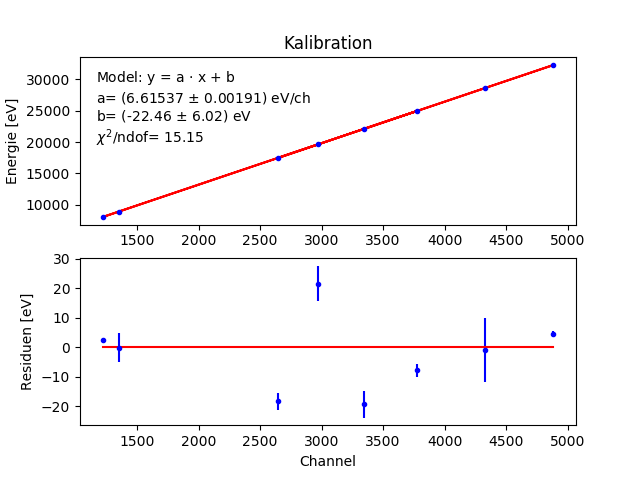
\includegraphics[scale=0.8]{Bilder/roentgen/Kalibration/linReg.png}
\caption{Energiekalibration durch lineare Regression der bekannten Peaks.}
\label{fig:röntgen_linReg}
\end{figure}

An diese acht Punkte wird nun eine lineare Regression der Form
\begin{equation*}
E (\textrm{ch}) = a \cdot \textrm{ch} + b
\end{equation*}
durchgeführt. Das Ergebnis ist in Abbildung \ref{fig:röntgen_linReg} gezeigt. Es wurde in eV gerechnet. Das $\chi ^2$/ndof von 15.15 deutet darauf hin, dass die Fehler unterschätzt sind.

\subsection{Einfluss der angelegten Hochspannung an die Röntgenröhre}

\begin{figure}
\centering
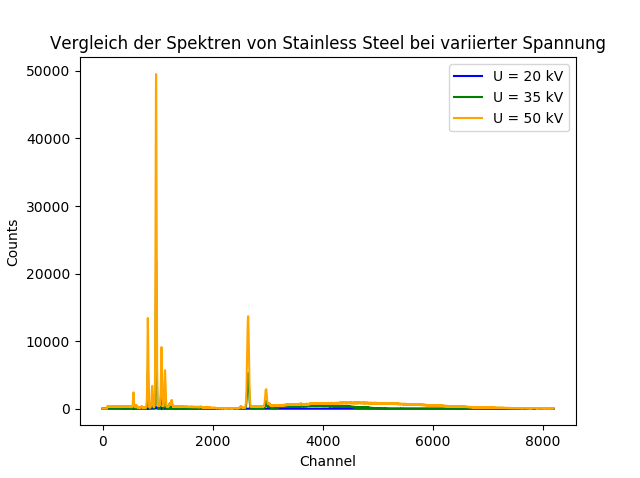
\includegraphics[scale=0.8]{Bilder/roentgen/Spannung/Gesamt.png}
\caption{Übereinandergelegte Messungen mit unterschiedlichen Spannung im gesamten Spektrum.}
\label{fig:spannung_gesamt}
\end{figure}

\begin{figure}
\centering
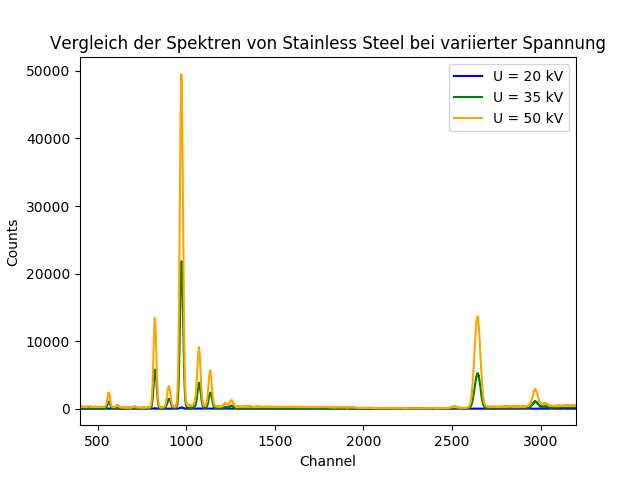
\includegraphics[scale=0.8]{Bilder/roentgen/Spannung/Ausschnitt.png}
\caption{Übereinandergelegte Messungen mit unterschiedlichen Spannung in einem Teil des Spektrum.}
\label{fig:spannung_ausschnitt}
\end{figure}

Die Röntgenröhre arbeitet mit einem Heizstrom zur Erzeugung thermischer Elektronen und einer Hochspannung zur Beschleunigung dieser auf das zu untersuchende Objekt. Die Energie, die diese Elektronen haben, wenn sie auf das Target treffen ist abhängig von der angelegten Hochspannung. Von dieser Energie hingegen ist abhängig, welche Phänomene beobachtet werden können. Abbildung \ref{fig:spannung_gesamt} zeigt die Messungen mit den unterschiedlichen Spannungen übereinandergelegt. In diesem Bild ist nur ein geringfügiger Unterschied zwischen den Messungen im Untergrund zu erkennen. Betrachtet man allerdings nur einen Teil des Spektrums, in dem die Peaks besser zu sehen sind, wie in Abbildung \ref{fig:spannung_ausschnitt}, werden die Unterschiede deutlicher. Die Höhe der Peaks sind bei einer eingestellten Spannung von \SI{35}{kV} deutlich niedriger als bei \SI{50}{kV}, wohingegen sie bei \SI{20}{kV} kaum noch erkennbar sind.

\subsection{Einfluss der PUR}

\begin{figure}
\centering
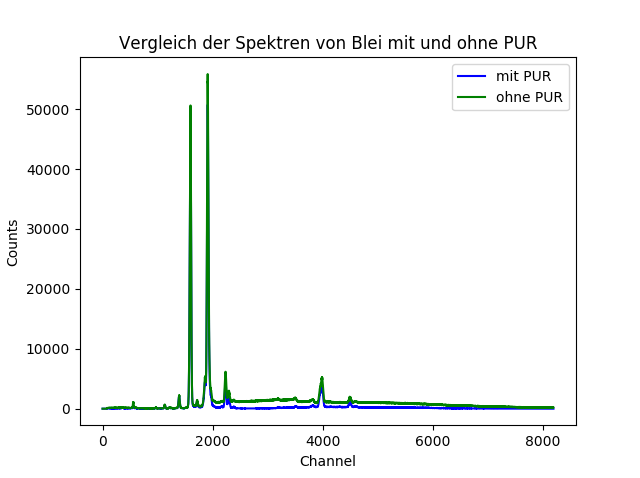
\includegraphics[scale=0.8]{Bilder/roentgen/PUR/Gesamt.png}
\caption{Übereinandergelegte Messungen mit und ohne Pile-up Rejection über das gesamte Spektrum.}
\label{fig:PUR_gesamt}
\end{figure}

\begin{figure}
\centering
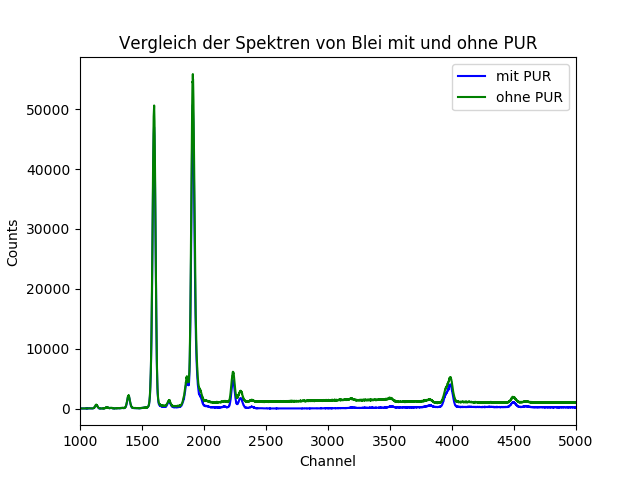
\includegraphics[scale=0.8]{Bilder/roentgen/PUR/Ausschnitt.png}
\caption{Übereinandergelegte Messungen mit und ohne Pile-up Rejection über einen Ausschnitt des Spektrum.}
\label{fig:PUR_ausschnitt}
\end{figure}

Die Pile-up Rejection (PUR) unterdrückt Pulse, die in der Totzeit des Detektors gemessen werden. Diese Pulse, die in der Totzeit gemessen werden, können keine physikalischen Messereignisse sein, daher ist die Unterdrückung dieser Pulse physikalisch sinnvoll. Da diese Unterdrückung in der Umsetzung nicht immer einfach ist, lohnt es sich, den Unterschied zwischen der Messung mit und ohne PUR näher zu betrachten. Abbildung \ref{fig:PUR_gesamt} zeigt übereinandergelegt diese Messungen für den Bleiblock. In diesem Bild ist erkennbar, dass der größte Unterschied zwischen den beiden Messungen im Bereich hinter den hohen Peaks liegt und dass der Unterschied ein kontinuierlicher Untergrund ist. Dies ist in Abbildung \ref{fig:PUR_ausschnitt}, in dem ein kleinerer Ausschnitt des Spektrums gezeigt ist, gut erkennbar.

\subsection{Auswertung unbekannter Proben}
\subsection{Energieauflösung}

\begin{table}
\centering
\begin{tabular}{|c|c|}
\hline 
Peakenergie [\si{eV}] & Full Width Half Maximum [\si{eV}] \\ 
\hline 
8045.8 $\pm$ 2.7 & 136.7 $\pm$ 6.3 \\ 
\hline
8903.0 $\pm$ 3.2 & 146.6 $\pm$ 7.6 \\ 
\hline
17460.3 $\pm$ 5.1 & 226 $\pm$ 12 \\ 
\hline
19625.4 $\pm$ 6.5 & 212 $\pm$ 15 \\ 
\hline
22120.2 $\pm$ 6.5 & 293 $\pm$ 15 \\ 
\hline
24951.3 $\pm$ 7.9 & 231 $\pm$ 19 \\ 
\hline
28618.4 $\pm$ 8.3 & 265 $\pm$ 20 \\ 
\hline
32290.8 $\pm$ 9.3 & 285 $\pm$ 22 \\ 
\hline
\end{tabular} 
\caption{Peakenergie und zugehörige Full Width Half Maxima.}
\label{tab:roentgen_energieaufloesung}
\end{table}

Zur Bestimmung der Energieauflösung werden die Peaks verwendet, die auch zur Kalibration verwendet werden. Dabei werden die Gaußanpassungen an die Peaks nach der Umrechnung der Kanäle auf Energie. Das Full Width Half Maximum (FWHM) bestimmt sich aus dem Breitenparameter aus der Gaußanpassung $\Delta$ gemäß:
\begin{equation*}
\textrm{FWHM} = 2 \cdot \sqrt{2 \cdot \ln(2)} \cdot \Delta
\end{equation*}
Entsprechend berechnet sich der Fehler über:
\begin{equation*}
\sigma _\textrm{FWHM} = 2 \cdot \sqrt{2 \cdot \ln(2)} \cdot \sigma _\Delta
\end{equation*}
Die Fehler auf die Breitenparameter und die Peakpositionen kommen aus der Anpassung. \\
Wegen des erwarteten Zusammenhangs $\Delta E \propto \sqrt{E}$ wird die Energieauflösung $\Delta E$ gegen die Wurzel der Energie aufgetragen. Der Fehler bestimmt sich zu:
\begin{equation*}
\sigma _{\sqrt{E}} = \dfrac{\sigma _E}{2 \cdot \sqrt{E}}
\end{equation*}
Tabelle \ref{tab:roentgen_energieaufloesung} zeigt die dadurch entstehenden Datenpunkte. An diese Punkte kann nun zur Überprüfung des Zusammenhang eine Transformation und dann eine lineare Regression durchgeführt werden. Diese ist in Abbildung \ref{fig:roentgen_energieaufloesung} gezeigt. Das $\chi ^2$/ndof von 2.71 deutet auf eine verhältnismäßig gute Anpassung, sodass der Zusammenhang $\Delta E \propto \sqrt{E}$ als bestätigt betrachtet werden kann, auch wenn hier mit insgesamt 8 Datenpunkten keine große Statistik gegeben ist.

\begin{figure}
\centering
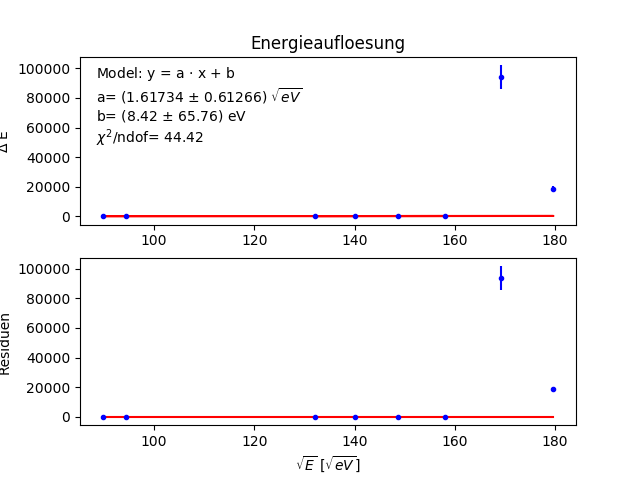
\includegraphics[scale=0.8]{Bilder/Energieaufloesung/roentgen_gesamt.png}
\caption{Lineare Regression an die Full Width Half Maxima und die Energien der Peaks.}
\label{fig:roentgen_energieaufloesung}
\end{figure}

\section{Fazit}
Die Untersuchung des Einflusses der Spannung hat den erwarteten Zusammenhang ergeben, dass die Peaks bei \SI{20}{kV} nicht, bei \SI{35}{kV} kaum und bei \SI{50}{kV} gut erkennbar sind. \\
Die Untersuchung des Einflusses der Pile-up Rejection hat ergeben, dass sich die Peaks in Position, Höhe und Breite gar nicht oder nur minimal verändern, wenn die PUR eingeschaltet ist. Daher kann davon ausgegangen werden, dass die Messungen mit und ohne PUR in der Auswertung gleiche Ergebnisse liefern. \\
Bei der Bestimmung der Energieauflösung konnte mittels einer linearen Regression bei geeigneter Auftragung der Zusammenhang $\Delta E \propto \sqrt{E}$ verifiziert werden. Die linearen Anpassungen haben dabei mit $\chi ^2$/ndof von 2.98 und 2.71 gut funktioniert.


\newpage 
\section{Anhang}
\subsection{Kalibration $\alpha$-Quelle}
\begin{figure}[H]
\centering
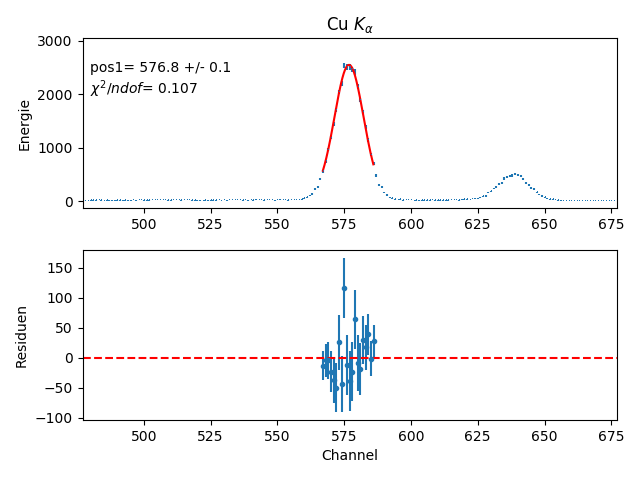
\includegraphics[scale=0.8]{Bilder/alpha/cu_alpha_1.png}
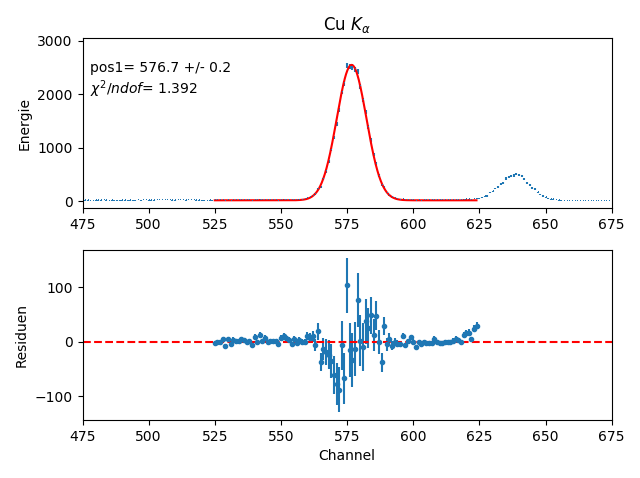
\includegraphics[scale=0.8]{Bilder/alpha/cu_alpha_2.png}
\caption{Alle für dei Kalibration aufgenommenen Spektren.}
\label{fig:kal_alles}
\end{figure}
\begin{figure}[H]
\centering
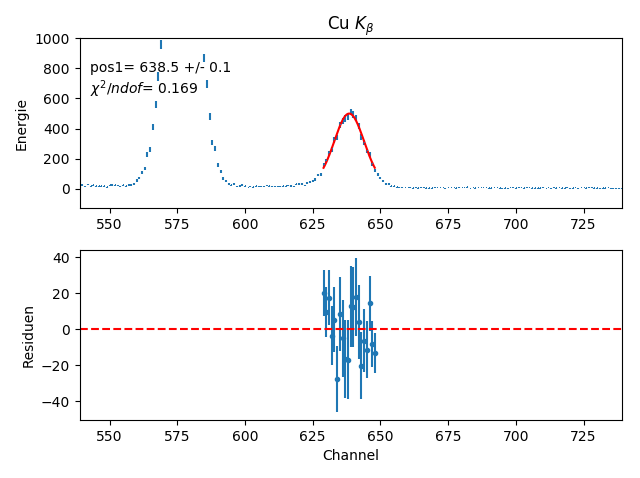
\includegraphics[scale=0.8]{Bilder/alpha/cu_beta_1.png}
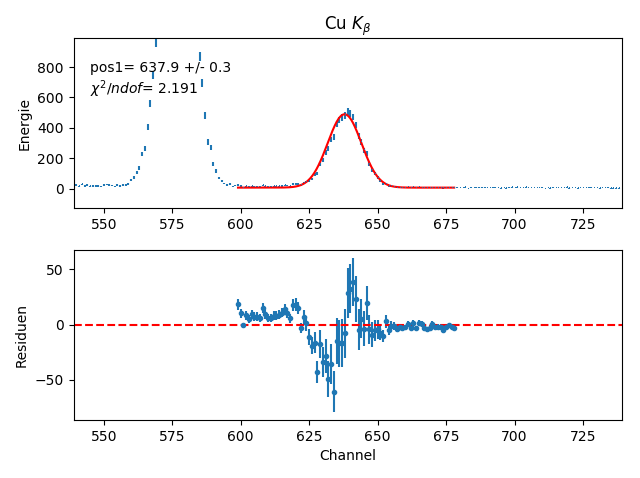
\includegraphics[scale=0.8]{Bilder/alpha/cu_beta_2.png}
\caption{Alle für dei Kalibration aufgenommenen Spektren.}
\label{fig:kal_alles}
\end{figure}

\begin{figure}[H]
\centering
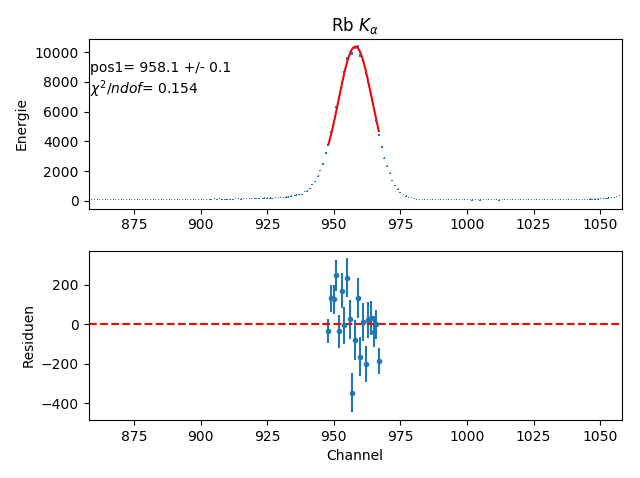
\includegraphics[scale=0.8]{Bilder/alpha/rb_alpha_1.png}
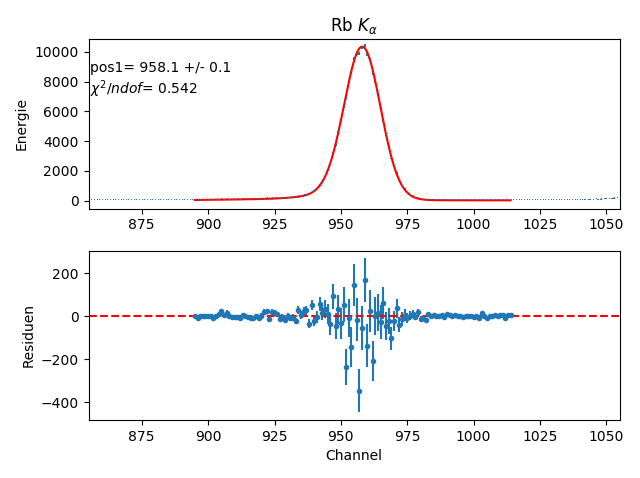
\includegraphics[scale=0.8]{Bilder/alpha/rb_alpha_2.png}
\caption{Alle für dei Kalibration aufgenommenen Spektren.}
\label{fig:kal_alles}
\end{figure}
\begin{figure}[H]
\centering
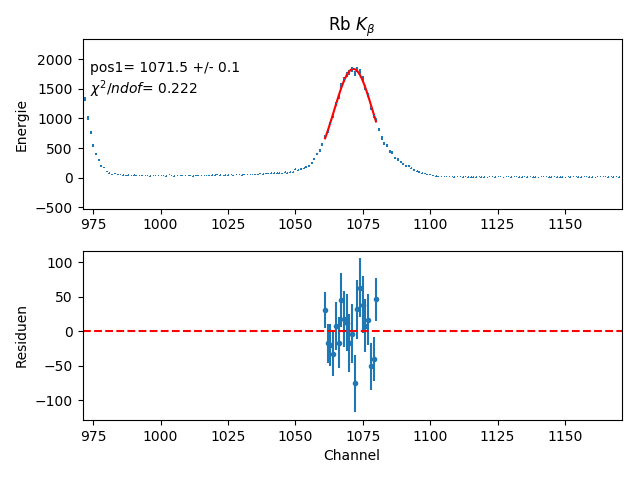
\includegraphics[scale=0.8]{Bilder/alpha/rb_beta_1.png}
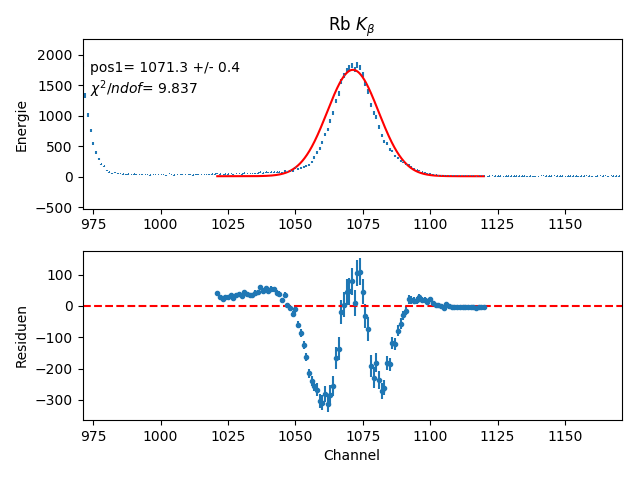
\includegraphics[scale=0.8]{Bilder/alpha/rb_beta_2.png}
\caption{Alle für dei Kalibration aufgenommenen Spektren.}
\label{fig:kal_alles}
\end{figure}

\begin{figure}[H]
\centering
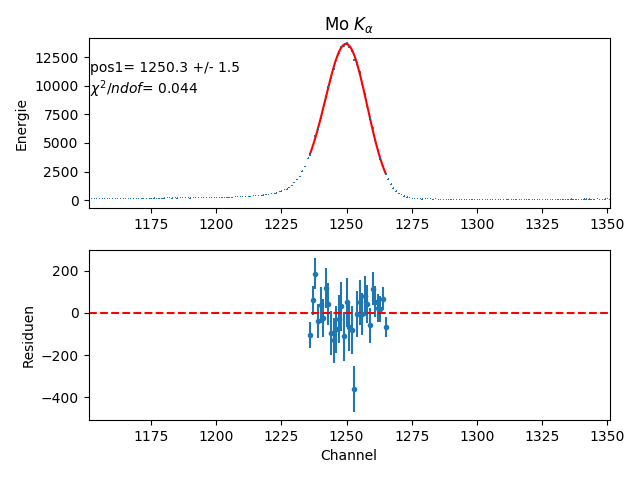
\includegraphics[scale=0.8]{Bilder/alpha/mo_alpha_1.png}
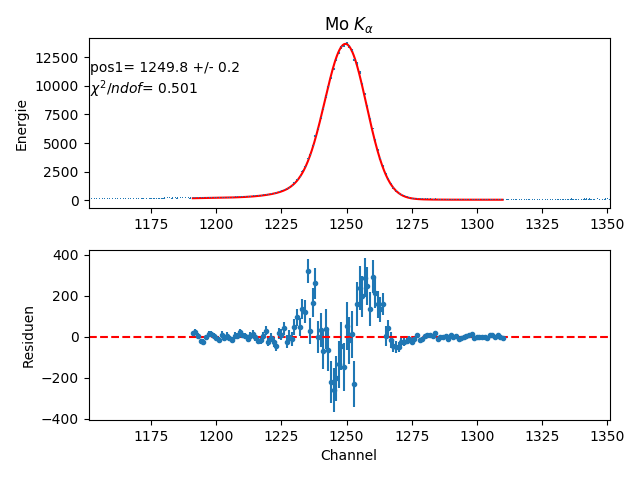
\includegraphics[scale=0.8]{Bilder/alpha/mo_alpha_2.png}
\caption{Alle für dei Kalibration aufgenommenen Spektren.}
\label{fig:kal_alles}
\end{figure}
\begin{figure}[H]
\centering
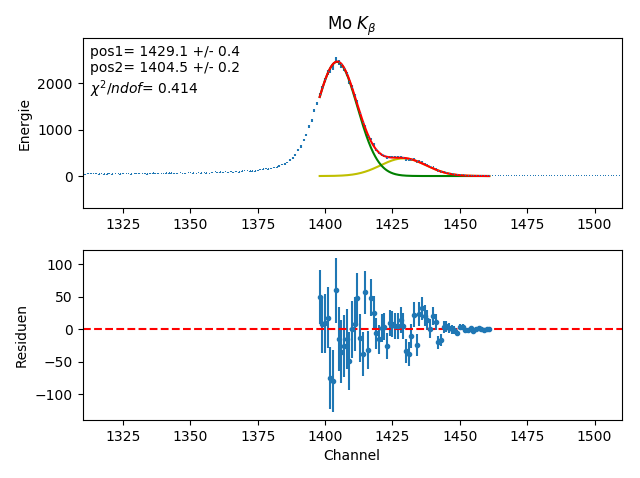
\includegraphics[scale=0.8]{Bilder/alpha/mo_beta_1.png}
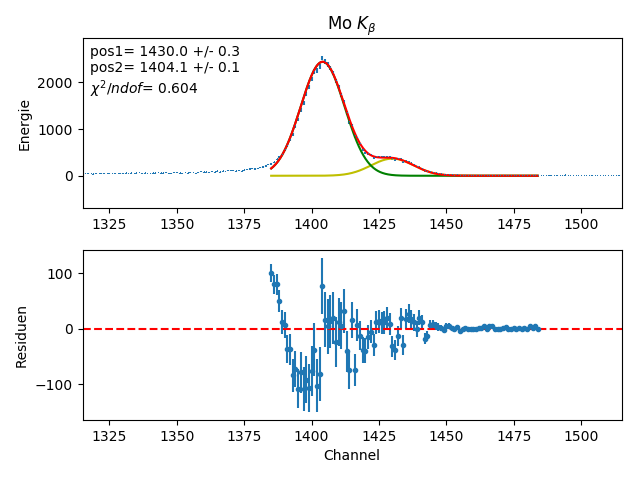
\includegraphics[scale=0.8]{Bilder/alpha/mo_beta_2.png}
\caption{Alle für dei Kalibration aufgenommenen Spektren.}
\label{fig:kal_alles}
\end{figure}

\begin{figure}[H]
\centering
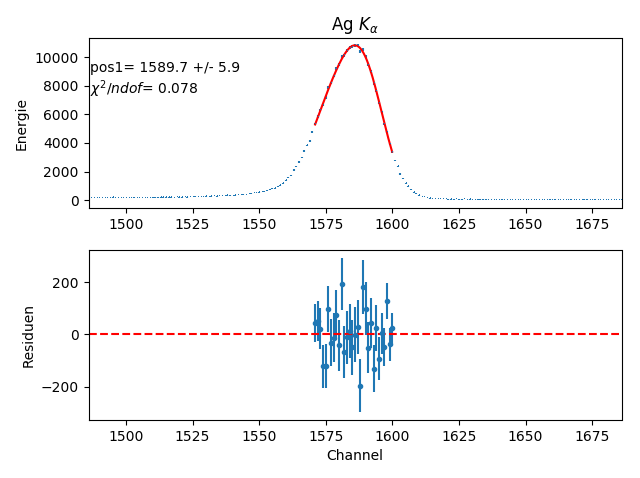
\includegraphics[scale=0.8]{Bilder/alpha/ag_alpha_1.png}
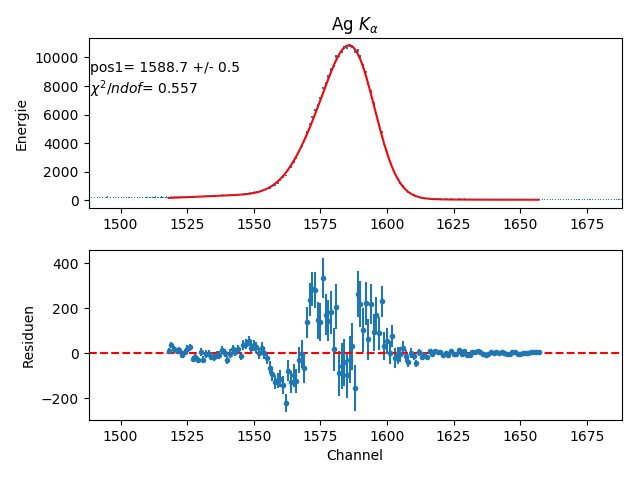
\includegraphics[scale=0.8]{Bilder/alpha/ag_alpha_2.png}
\caption{Alle für dei Kalibration aufgenommenen Spektren.}
\label{fig:kal_alles}
\end{figure}
\begin{figure}[H]
\centering
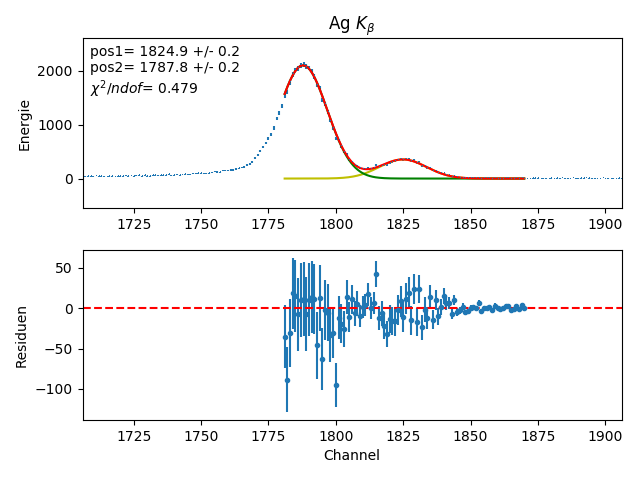
\includegraphics[scale=0.8]{Bilder/alpha/ag_beta_1.png}
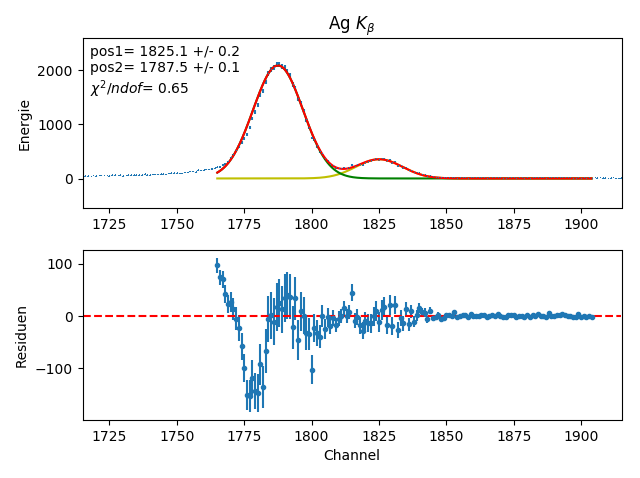
\includegraphics[scale=0.8]{Bilder/alpha/ag_beta_2.png}
\caption{Alle für dei Kalibration aufgenommenen Spektren.}
\label{fig:kal_alles}
\end{figure}

\begin{figure}[H]
\centering
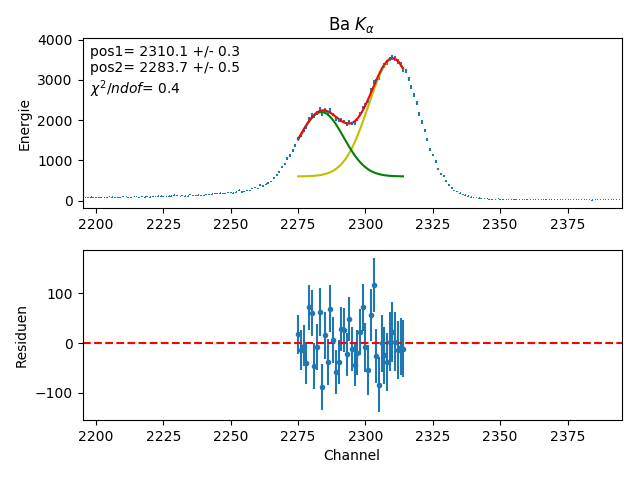
\includegraphics[scale=0.8]{Bilder/alpha/ba_alpha_1.png}
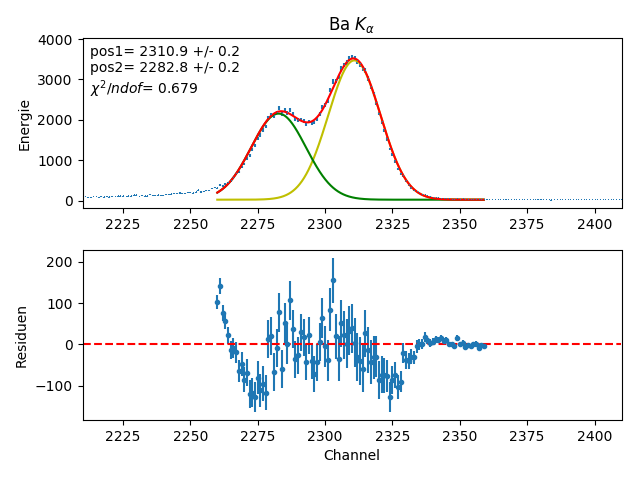
\includegraphics[scale=0.8]{Bilder/alpha/ba_alpha_2.png}
\caption{Alle für dei Kalibration aufgenommenen Spektren.}
\label{fig:kal_alles}
\end{figure}
\begin{figure}[H]
\centering
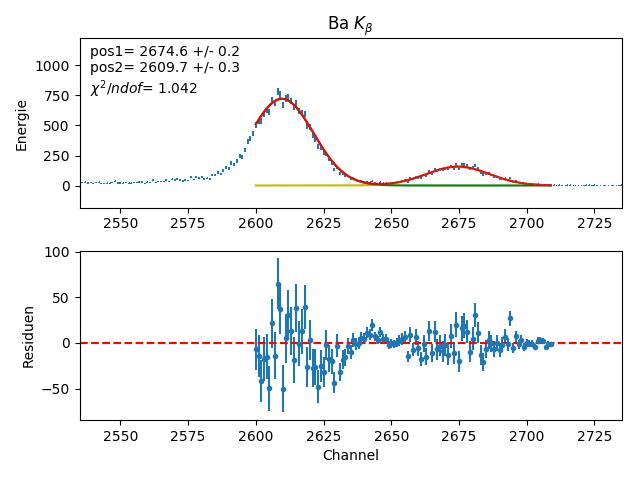
\includegraphics[scale=0.8]{Bilder/alpha/ba_beta_1.png}
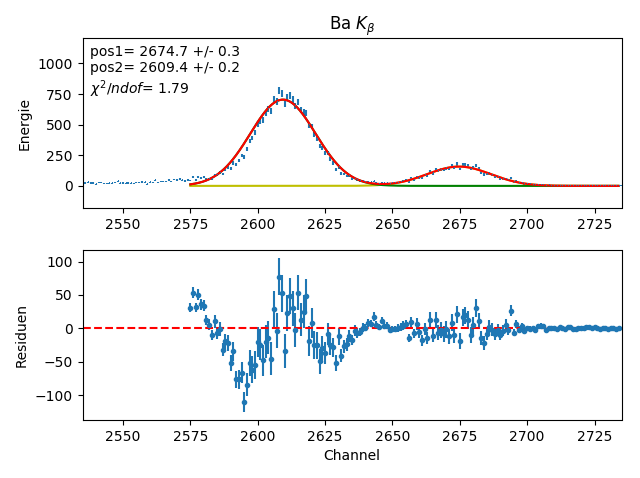
\includegraphics[scale=0.8]{Bilder/alpha/ba_beta_2.png}
\caption{Alle für dei Kalibration aufgenommenen Spektren.}
\label{fig:kal_alles}
\end{figure}

\begin{figure}[H]
\centering
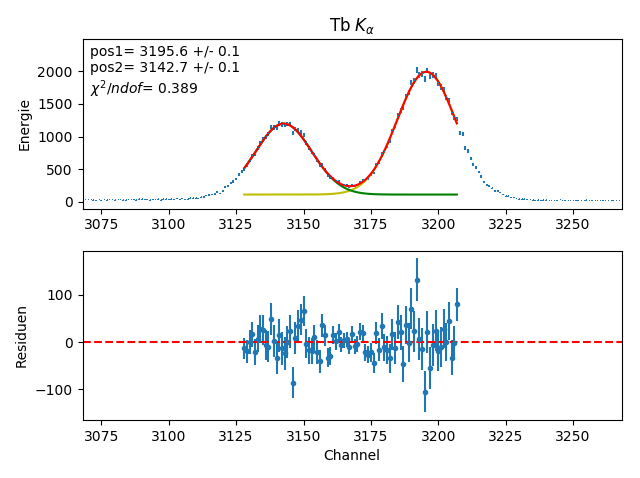
\includegraphics[scale=0.8]{Bilder/alpha/tb_alpha_1.png}
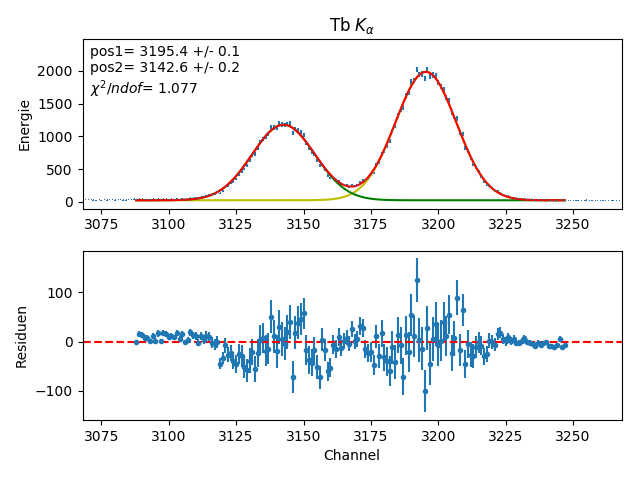
\includegraphics[scale=0.8]{Bilder/alpha/tb_alpha_2.png}
\caption{Alle für dei Kalibration aufgenommenen Spektren.}
\label{fig:kal_alles}
\end{figure}
\begin{figure}[H]
\centering
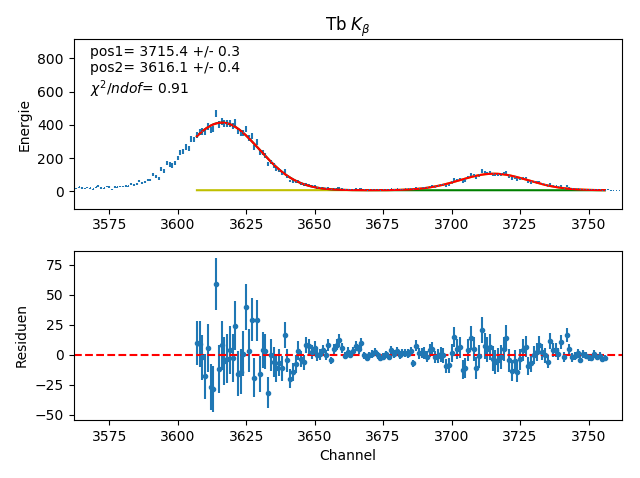
\includegraphics[scale=0.8]{Bilder/alpha/tb_beta_1.png}
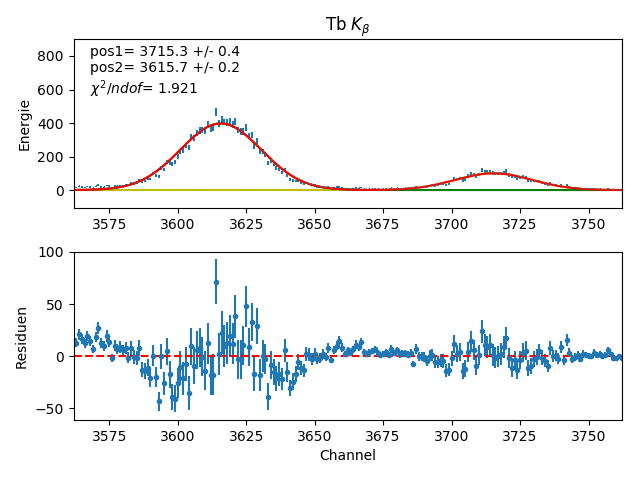
\includegraphics[scale=0.8]{Bilder/alpha/tb_beta_2.png}
\caption{Alle für dei Kalibration aufgenommenen Spektren.}
\label{fig:kal_alles}
\end{figure}

\subsection{Unbekannte Proben Röntgenquelle}
\subsubsection{Blei}
\begin{figure}[H]
\centering
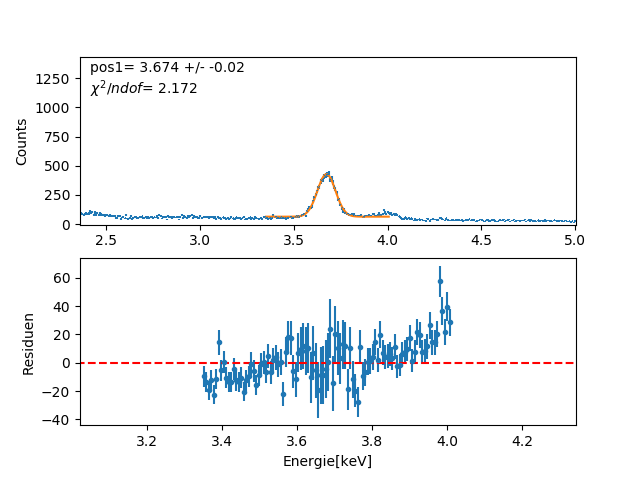
\includegraphics[scale=0.49]{Bilder/roentgen_spektren/blei/pb1_1.png}
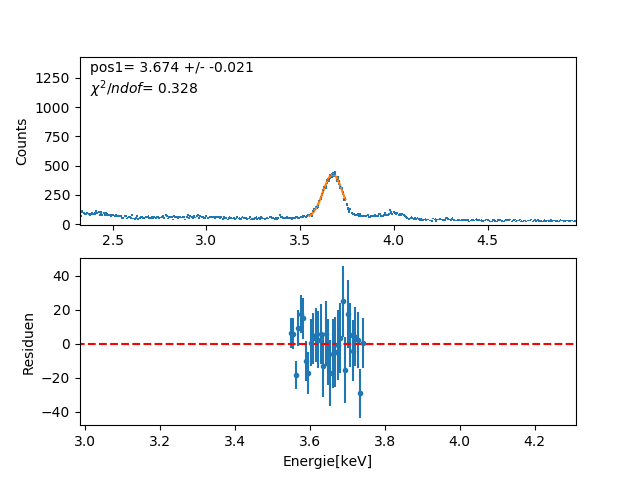
\includegraphics[scale=0.49]{Bilder/roentgen_spektren/blei/pb1_2.png}
\caption{Messung von Blei Peak1}
\end{figure}

\begin{figure}[H]
\centering
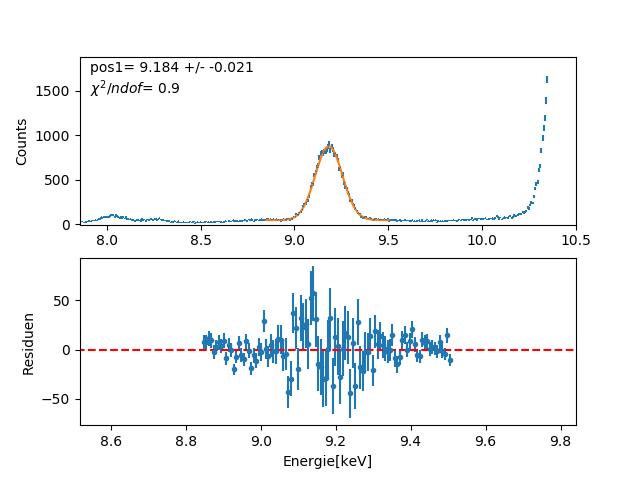
\includegraphics[scale=0.49]{Bilder/roentgen_spektren/blei/pb2_1.png}
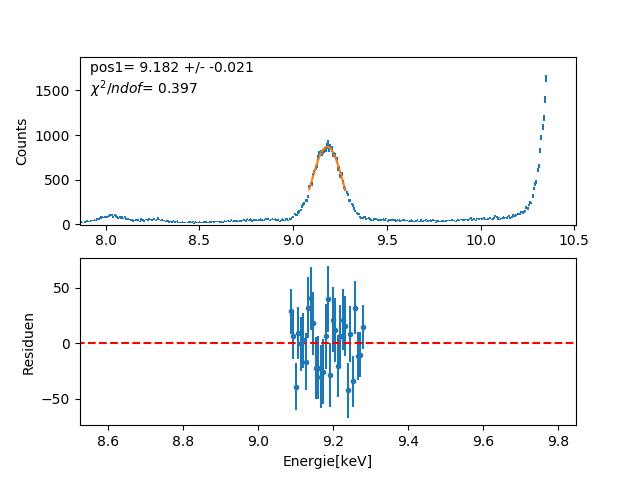
\includegraphics[scale=0.49]{Bilder/roentgen_spektren/blei/pb2_2.png}
\caption{Messung von Blei Peak2}
\end{figure}

\begin{figure}[H]
\centering
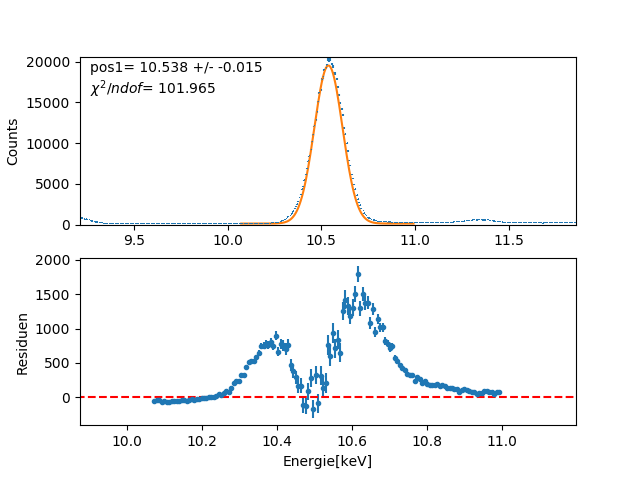
\includegraphics[scale=0.49]{Bilder/roentgen_spektren/blei/pb3_1.png}
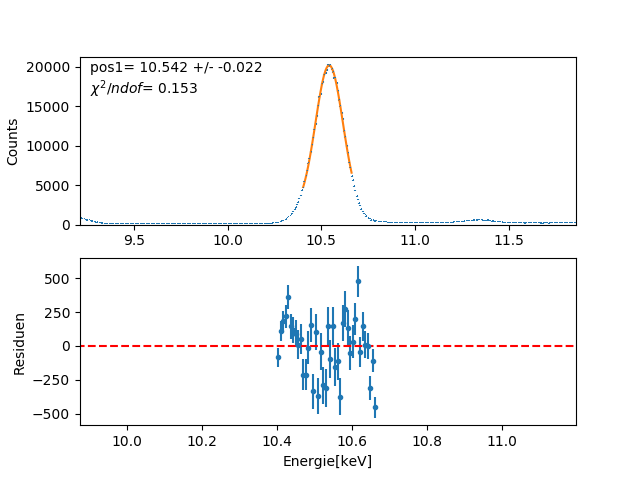
\includegraphics[scale=0.49]{Bilder/roentgen_spektren/blei/pb3_2.png}
\caption{Messung von Blei Peak3}
\end{figure}

\begin{figure}[H]
\centering
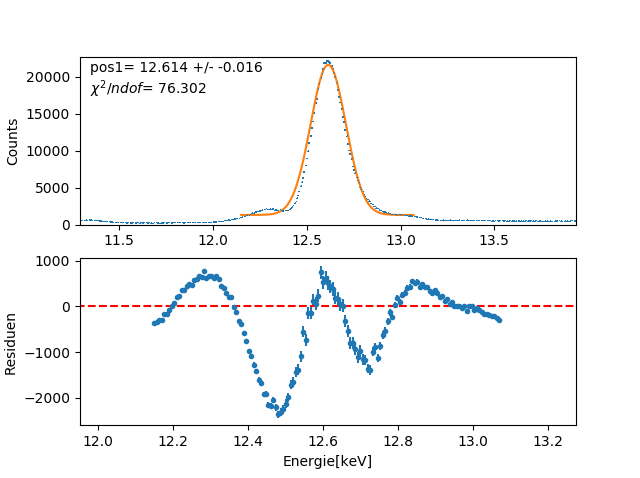
\includegraphics[scale=0.49]{Bilder/roentgen_spektren/blei/pb4_1.png}
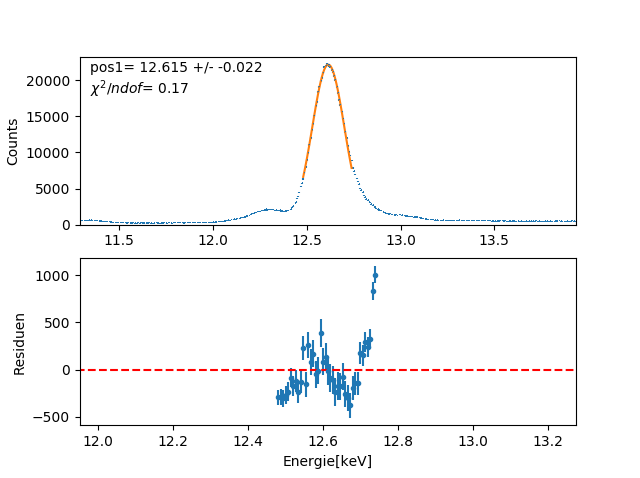
\includegraphics[scale=0.49]{Bilder/roentgen_spektren/blei/pb4_2.png}
\caption{Messung von Blei Peak4}
\end{figure}

\begin{figure}[H]
\centering
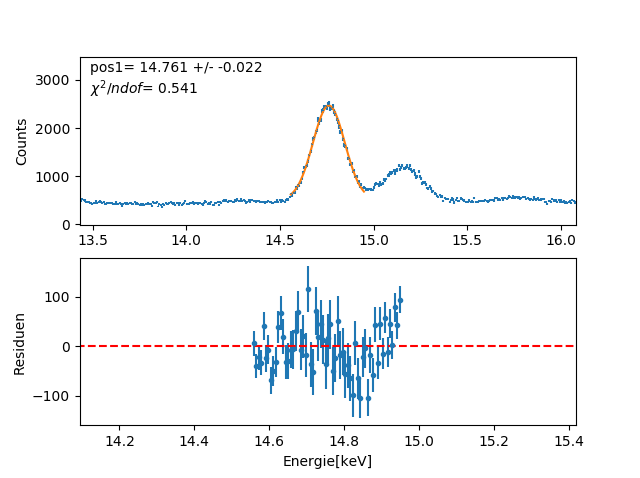
\includegraphics[scale=0.49]{Bilder/roentgen_spektren/blei/pb5_1.png}
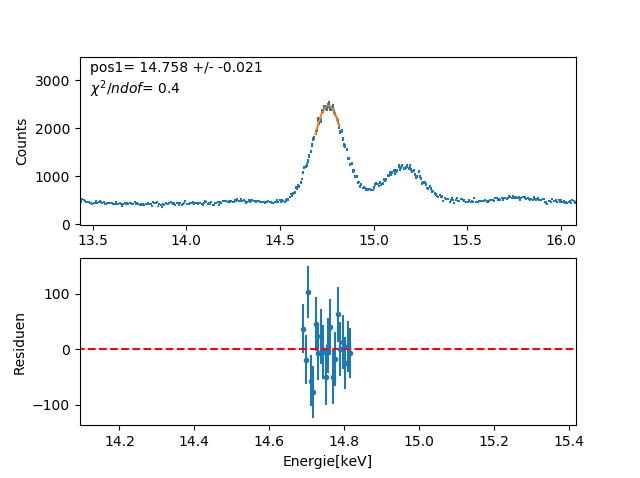
\includegraphics[scale=0.49]{Bilder/roentgen_spektren/blei/pb5_2.png}
\caption{Messung von Blei Peak5}
\end{figure}

\begin{figure}[H]
\centering
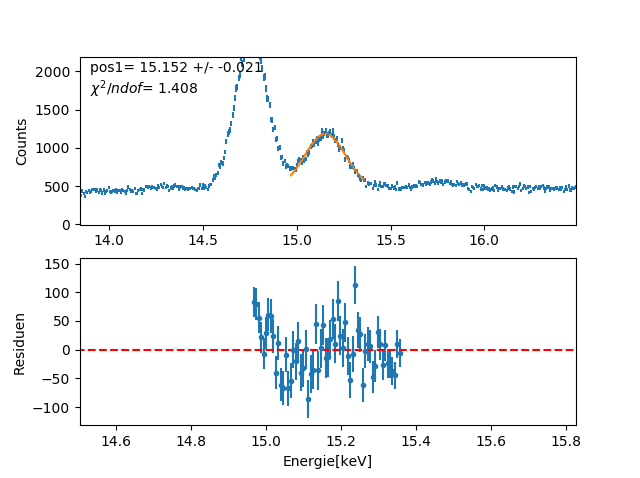
\includegraphics[scale=0.49]{Bilder/roentgen_spektren/blei/pb6_1.png}
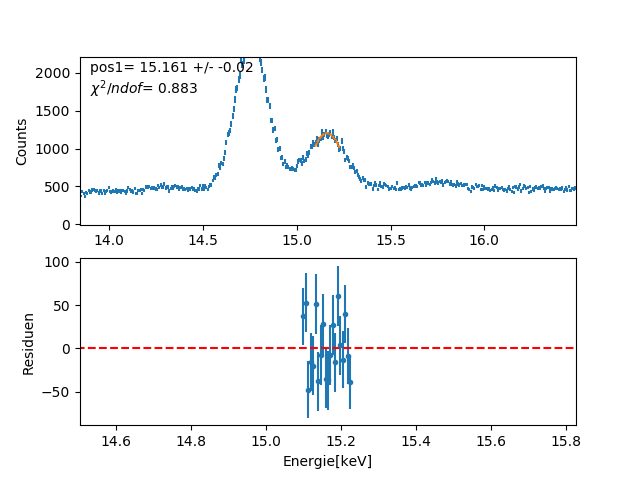
\includegraphics[scale=0.49]{Bilder/roentgen_spektren/blei/pb6_2.png}
\caption{Messung von Blei Peak6}
\end{figure}

\begin{figure}[H]
\centering
\includegraphics[scale=0.49]{Bilder/roentgen_spektren/blei/pb7_1.png}
\includegraphics[scale=0.49]{Bilder/roentgen_spektren/blei/pb7_2.png}
\caption{Messung von Blei Peak7}
\end{figure}

\begin{figure}[H]
\centering
\includegraphics[scale=0.49]{Bilder/roentgen_spektren/blei/pb8_1.png}
\includegraphics[scale=0.49]{Bilder/roentgen_spektren/blei/pb8_2.png}
\caption{Messung von Blei Peak8}
\end{figure}

\newpage
\subsubsection{PC-Chip}
\begin{figure}[H]
\centering
\includegraphics[scale=0.49]{Bilder/roentgen_spektren/chip/chip1_1.png}
\includegraphics[scale=0.49]{Bilder/roentgen_spektren/chip/chip1_2.png}
\caption{Messung des Chips Peak1}
\end{figure}

\begin{figure}[H]
\centering
\includegraphics[scale=0.49]{Bilder/roentgen_spektren/chip/chip2_1.png}
\includegraphics[scale=0.49]{Bilder/roentgen_spektren/chip/chip2_2.png}
\caption{Messung des Chips Peak2}
\end{figure}

\begin{figure}[H]
\centering
\includegraphics[scale=0.49]{Bilder/roentgen_spektren/chip/chip3_1.png}
\includegraphics[scale=0.49]{Bilder/roentgen_spektren/chip/chip3_2.png}
\caption{Messung des Chips Peak3}
\end{figure}

\begin{figure}[H]
\centering
\includegraphics[scale=0.49]{Bilder/roentgen_spektren/chip/chip4_1.png}
\includegraphics[scale=0.49]{Bilder/roentgen_spektren/chip/chip4_2.png}
\caption{Messung des Chips Peak4}
\end{figure}

\begin{figure}[H]
\centering
\includegraphics[scale=0.49]{Bilder/roentgen_spektren/chip/chip5_1.png}
\includegraphics[scale=0.49]{Bilder/roentgen_spektren/chip/chip5_2.png}
\caption{Messung des Chips Peak5}
\end{figure}

\begin{figure}[H]
\centering
\includegraphics[scale=0.49]{Bilder/roentgen_spektren/chip/chip6_1.png}
\includegraphics[scale=0.49]{Bilder/roentgen_spektren/chip/chip6_2.png}
\caption{Messung des Chips Peak6}
\end{figure}

\begin{figure}[H]
\centering
\includegraphics[scale=0.49]{Bilder/roentgen_spektren/chip/chip7_1.png}
\includegraphics[scale=0.49]{Bilder/roentgen_spektren/chip/chip7_2.png}
\caption{Messung des Chips Peak7}
\end{figure}

\begin{figure}[H]
\centering
\includegraphics[scale=0.49]{Bilder/roentgen_spektren/chip/chip8_1.png}
\includegraphics[scale=0.49]{Bilder/roentgen_spektren/chip/chip8_2.png}
\caption{Messung des Chips Peak8}
\end{figure}

\begin{figure}[H]
\centering
\includegraphics[scale=0.49]{Bilder/roentgen_spektren/chip/chip9_1.png}
\includegraphics[scale=0.49]{Bilder/roentgen_spektren/chip/chip9_2.png}
\caption{Messung des Chips Peak9}
\end{figure}

\begin{figure}[H]
\centering
\includegraphics[scale=0.49]{Bilder/roentgen_spektren/chip/chip10_1.png}
\includegraphics[scale=0.49]{Bilder/roentgen_spektren/chip/chip10_2.png}
\caption{Messung des Chips Peak10}
\end{figure}

\begin{figure}[H]
\centering
\includegraphics[scale=0.49]{Bilder/roentgen_spektren/chip/chip11_1.png}
\includegraphics[scale=0.49]{Bilder/roentgen_spektren/chip/chip11_2.png}
\caption{Messung des Chips Peak11}
\end{figure}

\newpage
\subsubsection{2-Dinar-Münze}
\begin{figure}[H]
\centering
\includegraphics[scale=0.49]{Bilder/roentgen_spektren/denar/den1_1.png}
\includegraphics[scale=0.49]{Bilder/roentgen_spektren/denar/den1_2.png}
\caption{Messung der 2-Dinar-Münze Peak1}
\end{figure}

\begin{figure}[H]
\centering
\includegraphics[scale=0.49]{Bilder/roentgen_spektren/denar/den2_1.png}
\includegraphics[scale=0.49]{Bilder/roentgen_spektren/denar/den2_2.png}
\caption{Messung der 2-Dinar-Münze Peak2}
\end{figure}

\begin{figure}[H]
\centering
\includegraphics[scale=0.49]{Bilder/roentgen_spektren/denar/den3_1.png}
\includegraphics[scale=0.49]{Bilder/roentgen_spektren/denar/den3_2.png}
\caption{Messung der 2-Dinar-Münze Peak3}
\end{figure}

\begin{figure}[H]
\centering
\includegraphics[scale=0.49]{Bilder/roentgen_spektren/denar/den4_1.png}
\includegraphics[scale=0.49]{Bilder/roentgen_spektren/denar/den4_2.png}
\caption{Messung der 2-Dinar-Münze Peak4}
\end{figure}

\begin{figure}[H]
\centering
\includegraphics[scale=0.49]{Bilder/roentgen_spektren/denar/den5_1.png}
\includegraphics[scale=0.49]{Bilder/roentgen_spektren/denar/den5_2.png}
\caption{Messung der 2-Dinar-Münze Peak5}
\end{figure}

\begin{figure}[H]
\centering
\includegraphics[scale=0.49]{Bilder/roentgen_spektren/denar/den6_1.png}
\includegraphics[scale=0.49]{Bilder/roentgen_spektren/denar/den6_2.png}
\caption{Messung der 2-Dinar-Münze Peak6}
\end{figure}

\begin{figure}[H]
\centering
\includegraphics[scale=0.49]{Bilder/roentgen_spektren/denar/den7_1.png}
\includegraphics[scale=0.49]{Bilder/roentgen_spektren/denar/den7_2.png}
\caption{Messung der 2-Dinar-Münze Peak7}
\end{figure}

\begin{figure}[H]
\centering
\includegraphics[scale=0.49]{Bilder/roentgen_spektren/denar/den8_1.png}
\includegraphics[scale=0.49]{Bilder/roentgen_spektren/denar/den8_2.png}
\caption{Messung der 2-Dinar-Münze Peak8}
\end{figure}

\newpage
\subsubsection{Magnet}
\begin{figure}[H]
\centering
\includegraphics[scale=0.49]{Bilder/roentgen_spektren/magnet/mag1_1.png}
\includegraphics[scale=0.49]{Bilder/roentgen_spektren/magnet/mag1_2.png}
\caption{Messung des Magneten Peak1}
\end{figure}

\begin{figure}[H]
\centering
\includegraphics[scale=0.49]{Bilder/roentgen_spektren/magnet/mag2_1.png}
\includegraphics[scale=0.49]{Bilder/roentgen_spektren/magnet/mag2_2.png}
\caption{Messung des Magneten Peak2}
\end{figure}

\begin{figure}[H]
\centering
\includegraphics[scale=0.49]{Bilder/roentgen_spektren/magnet/mag3_1.png}
\includegraphics[scale=0.49]{Bilder/roentgen_spektren/magnet/mag3_2.png}
\caption{Messung des Magneten Peak3}
\end{figure}

\begin{figure}[H]
\centering
\includegraphics[scale=0.49]{Bilder/roentgen_spektren/magnet/mag4_1.png}
\includegraphics[scale=0.49]{Bilder/roentgen_spektren/magnet/mag4_2.png}
\caption{Messung des Magneten Peak4}
\end{figure}

\begin{figure}[H]
\centering
\includegraphics[scale=0.49]{Bilder/roentgen_spektren/magnet/mag5_1.png}
\includegraphics[scale=0.49]{Bilder/roentgen_spektren/magnet/mag5_2.png}
\caption{Messung des Magneten Peak5}
\end{figure}

\begin{figure}[H]
\centering
\includegraphics[scale=0.49]{Bilder/roentgen_spektren/magnet/mag6_1.png}
\includegraphics[scale=0.49]{Bilder/roentgen_spektren/magnet/mag6_2.png}
\caption{Messung des Magneten Peak6}
\end{figure}

\begin{figure}[H]
\centering
\includegraphics[scale=0.49]{Bilder/roentgen_spektren/magnet/mag7_1.png}
\includegraphics[scale=0.49]{Bilder/roentgen_spektren/magnet/mag7_2.png}
\caption{Messung des Magneten Peak7}
\end{figure}

\begin{figure}[H]
\centering
\includegraphics[scale=0.49]{Bilder/roentgen_spektren/magnet/mag8_1.png}
\includegraphics[scale=0.49]{Bilder/roentgen_spektren/magnet/mag8_2.png}
\caption{Messung des Magneten Peak8}
\end{figure}

\begin{figure}[H]
\centering
\includegraphics[scale=0.49]{Bilder/roentgen_spektren/magnet/mag9_1.png}
\includegraphics[scale=0.49]{Bilder/roentgen_spektren/magnet/mag9_2.png}
\caption{Messung des Magneten Peak9}
\end{figure}

\begin{figure}[H]
\centering
\includegraphics[scale=0.49]{Bilder/roentgen_spektren/magnet/mag10_1.png}
\includegraphics[scale=0.49]{Bilder/roentgen_spektren/magnet/mag10_2.png}
\caption{Messung des Magneten Peak10}
\end{figure}

\begin{figure}[H]
\centering
\includegraphics[scale=0.49]{Bilder/roentgen_spektren/magnet/mag11_1.png}
\includegraphics[scale=0.49]{Bilder/roentgen_spektren/magnet/mag11_2.png}
\caption{Messung des Magneten Peak11}
\end{figure}

\begin{figure}[H]
\centering
\includegraphics[scale=0.49]{Bilder/roentgen_spektren/magnet/mag12_1.png}
\includegraphics[scale=0.49]{Bilder/roentgen_spektren/magnet/mag12_2.png}
\caption{Messung des Magneten Peak12}
\end{figure}

\begin{figure}[H]
\centering
\includegraphics[scale=0.49]{Bilder/roentgen_spektren/magnet/mag13_1.png}
\includegraphics[scale=0.49]{Bilder/roentgen_spektren/magnet/mag13_2.png}
\caption{Messung des Magneten Peak13}
\end{figure}

\begin{figure}[H]
\centering
\includegraphics[scale=0.49]{Bilder/roentgen_spektren/magnet/mag14_1.png}
\includegraphics[scale=0.49]{Bilder/roentgen_spektren/magnet/mag14_2.png}
\caption{Messung des Magneten Peak14}
\end{figure}

\begin{figure}[H]
\centering
\includegraphics[scale=0.49]{Bilder/roentgen_spektren/magnet/mag15_1.png}
\includegraphics[scale=0.49]{Bilder/roentgen_spektren/magnet/mag15_2.png}
\caption{Messung des Magneten Peak15}
\end{figure}

\begin{figure}[H]
\centering
\includegraphics[scale=0.49]{Bilder/roentgen_spektren/magnet/mag16_1.png}
\includegraphics[scale=0.49]{Bilder/roentgen_spektren/magnet/mag16_2.png}
\caption{Messung des Magneten Peak16}
\end{figure}

\newpage
\subsubsection{10-Pfennig-Münze}
\begin{figure}[H]
\centering
\includegraphics[scale=0.49]{Bilder/roentgen_spektren/pfennig/pfen1_1.png}
\includegraphics[scale=0.49]{Bilder/roentgen_spektren/pfennig/pfen1_2.png}
\caption{Messung der 10-Pfennig-Münze Peak1}
\end{figure}

\begin{figure}[H]
\centering
\includegraphics[scale=0.49]{Bilder/roentgen_spektren/pfennig/pfen2_1.png}
\includegraphics[scale=0.49]{Bilder/roentgen_spektren/pfennig/pfen2_2.png}
\caption{Messung der 10-Pfennig-Münze Peak2}
\end{figure}

\begin{figure}[H]
\centering
\includegraphics[scale=0.49]{Bilder/roentgen_spektren/pfennig/pfen3_1.png}
\includegraphics[scale=0.49]{Bilder/roentgen_spektren/pfennig/pfen3_2.png}
\caption{Messung der 10-Pfennig-Münze Peak3}
\end{figure}

\begin{figure}[H]
\centering
\includegraphics[scale=0.49]{Bilder/roentgen_spektren/pfennig/pfen4_1.png}
\includegraphics[scale=0.49]{Bilder/roentgen_spektren/pfennig/pfen4_2.png}
\caption{Messung der 10-Pfennig-Münze Peak4}
\end{figure}

\begin{figure}[H]
\centering
\includegraphics[scale=0.49]{Bilder/roentgen_spektren/pfennig/pfen5_1.png}
\includegraphics[scale=0.49]{Bilder/roentgen_spektren/pfennig/pfen5_2.png}
\caption{Messung der 10-Pfennig-Münze Peak5}
\end{figure}

\begin{figure}[H]
\centering
\includegraphics[scale=0.49]{Bilder/roentgen_spektren/pfennig/pfen6_1.png}
\includegraphics[scale=0.49]{Bilder/roentgen_spektren/pfennig/pfen6_2.png}
\caption{Messung der 10-Pfennig-Münze Peak6}
\end{figure}

\begin{figure}[H]
\centering
\includegraphics[scale=0.49]{Bilder/roentgen_spektren/pfennig/pfen7_1.png}
\includegraphics[scale=0.49]{Bilder/roentgen_spektren/pfennig/pfen7_2.png}
\caption{Messung der 10-Pfennig-Münze Peak7}
\end{figure}

\begin{figure}[H]
\centering
\includegraphics[scale=0.49]{Bilder/roentgen_spektren/pfennig/pfen8_1.png}
\includegraphics[scale=0.49]{Bilder/roentgen_spektren/pfennig/pfen8_2.png}
\caption{Messung der 10-Pfennig-Münze Peak8}
\end{figure}

\newpage
\subsubsection{10-Rubel-Münze}
\begin{figure}[H]
\centering
\includegraphics[scale=0.49]{Bilder/roentgen_spektren/rubel/rub1_1.png}
\includegraphics[scale=0.49]{Bilder/roentgen_spektren/rubel/rub1_2.png}
\caption{Messung der 10-Rubel-Münze Peak1}
\end{figure}

\begin{figure}[H]
\centering
\includegraphics[scale=0.49]{Bilder/roentgen_spektren/rubel/rub3_1.png}
\includegraphics[scale=0.49]{Bilder/roentgen_spektren/rubel/rub3_2.png}
\caption{Messung der 10-Rubel-Münze Peak2}
\end{figure}

\begin{figure}[H]
\centering
\includegraphics[scale=0.49]{Bilder/roentgen_spektren/rubel/rub4_1.png}
\includegraphics[scale=0.49]{Bilder/roentgen_spektren/rubel/rub4_2.png}
\caption{Messung der 10-Rubel-Münze Peak3}
\end{figure}

\begin{figure}[H]
\centering
\includegraphics[scale=0.49]{Bilder/roentgen_spektren/rubel/rub5_1.png}
\includegraphics[scale=0.49]{Bilder/roentgen_spektren/rubel/rub5_2.png}
\caption{Messung der 10-Rubel-Münze Peak4}
\end{figure}

\begin{figure}[H]
\centering
\includegraphics[scale=0.49]{Bilder/roentgen_spektren/rubel/rub6_1.png}
\includegraphics[scale=0.49]{Bilder/roentgen_spektren/rubel/rub6_2.png}
\caption{Messung der 10-Rubel-Münze Peak5}
\end{figure}

\begin{figure}[H]
\centering
\includegraphics[scale=0.49]{Bilder/roentgen_spektren/rubel/rub7_1.png}
\includegraphics[scale=0.49]{Bilder/roentgen_spektren/rubel/rub7_2.png}
\caption{Messung der 10-Rubel-Münze Peak6}
\end{figure}

\begin{figure}[H]
\centering
\includegraphics[scale=0.49]{Bilder/roentgen_spektren/rubel/rub8_1.png}
\includegraphics[scale=0.49]{Bilder/roentgen_spektren/rubel/rub8_2.png}
\caption{Messung der 10-Rubel-Münze Peak7}
\end{figure}

\newpage
\subsubsection{Stainless Steel}
\begin{figure}[H]
\centering
\includegraphics[scale=0.49]{Bilder/roentgen_spektren/stahl/rub1_1.png}
\includegraphics[scale=0.49]{Bilder/roentgen_spektren/stahl/rub1_2.png}
\caption{Messung des Stainless Steel Peak1}
\end{figure}

\begin{figure}[H]
\centering
\includegraphics[scale=0.49]{Bilder/roentgen_spektren/stahl/rub2_1.png}
\includegraphics[scale=0.49]{Bilder/roentgen_spektren/stahl/rub2_2.png}
\caption{Messung des Stainless Steel Peak2}
\end{figure}

\begin{figure}[H]
\centering
\includegraphics[scale=0.49]{Bilder/roentgen_spektren/stahl/rub3_1.png}
\includegraphics[scale=0.49]{Bilder/roentgen_spektren/stahl/rub3_2.png}
\caption{Messung des Stainless Steel Peak3}
\end{figure}

\begin{figure}[H]
\centering
\includegraphics[scale=0.49]{Bilder/roentgen_spektren/stahl/rub4_1.png}
\includegraphics[scale=0.49]{Bilder/roentgen_spektren/stahl/rub4_2.png}
\caption{Messung des Stainless Steel Peak4}
\end{figure}

\begin{figure}[H]
\centering
\includegraphics[scale=0.49]{Bilder/roentgen_spektren/stahl/rub5_1.png}
\includegraphics[scale=0.49]{Bilder/roentgen_spektren/stahl/rub5_2.png}
\caption{Messung des Stainless Steel Peak5}
\end{figure}

\begin{figure}[H]
\centering
\includegraphics[scale=0.49]{Bilder/roentgen_spektren/stahl/rub6_1.png}
\includegraphics[scale=0.49]{Bilder/roentgen_spektren/stahl/rub6_2.png}
\caption{Messung des Stainless Steel Peak6}
\end{figure}

\begin{figure}[H]
\centering
\includegraphics[scale=0.49]{Bilder/roentgen_spektren/stahl/rub7_1.png}
\includegraphics[scale=0.49]{Bilder/roentgen_spektren/stahl/rub7_2.png}
\caption{Messung des Stainless Steel Peak7}
\end{figure}

\begin{figure}[H]
\centering
\includegraphics[scale=0.49]{Bilder/roentgen_spektren/stahl/rub8_1.png}
\includegraphics[scale=0.49]{Bilder/roentgen_spektren/stahl/rub8_2.png}
\caption{Messung des Stainless Steel Peak8}
\end{figure}


\end{document}
